\documentclass{ximera}

\graphicspath{{./graphics/}{./content/04_2_quadratic_forms/graphics/}}

\title{Quadratic Forms}
\author{Melissa Lynn}
\outcome{Identify and classify quadratic forms. Use Sylvester's theorem where appropriate.}

\begin{document}
\begin{abstract}
\end{abstract}
\maketitle

In order to better understand the behavior of multivariable functions, we would like to define some sort of second derivative for multivariable functions. For first derivatives, we have the gradient and derivative matrix filling the roles of derivatives for scalar-valued and vector-valued functions, respectively. Before we define the second derivative, we will try to understand second-order behavior in multivariable functions specifically. That is, we'll consider polynomials in $n$-variables that only terms of degree $2$, and determine how these polynomials behave.

Polynomials with this property are very important throughout mathematics, and they are called quadratic forms. You've frequently seen a quadratic form which arises from the length of a vector $\vec{x} = (x_1,...,x_n)$,
\[
\|\vec{x}\|^2 = x_1^2 + x_2^2 + \cdots + x_n^2.
\]

\section*{Quadratic Forms}

\begin{definition}
A \emph{quadratic form} in $\mathbb{R}^n$ is a polynomial $p:\mathbb{R}^n\rightarrow\mathbb{R}$ in which each term has total degree $2$. That is, it has the form
\begin{align*}
p(x_1,...,x_n) &= c_{11}x_1^2+c_{12}x_1x_2+c_{13}x_1x_3 + \cdots + c_{1n}x_1x_n\\
&\phantom{= c_{11}x_1^2}+c_{22}x_2^2\phantom{x_2}+c_{23}x_2x_3 + \cdots + c_{2n}x_2x_n\\
&\phantom{= c_{11}x_1^2+c_{12}x_1x_2}+c_{33}x_3^2\phantom{x_3} + \cdots + c_{3n}x_3x_n\\
&\phantom{= c_{11}x_1^2+c_{12}x_1x_2+c_{13}x_1x_3 +} \ddots \phantom{+} \vdots\\
&\phantom{= c_{11}x_1^2+c_{12}x_1x_2+c_{13}x_1x_3 + \cdots }+ c_{nn}x_n^2
\end{align*}
\end{definition}

\begin{example}
For example, the polynomials $x^2+2xy+y^2$ and $xy+yz-xz$ are quadratic forms.

On the other hand, $\sin(x^2)$ and $\frac{x^3}{y}$ are not quadratic forms, since they're not polynomials. Also, the polynomials $x^2+y^2-1$ and $(x+1)^2$ are not quadratic forms, since they include terms of degrees other than $2$
\end{example}

For any quadratic form \begin{align*}
p(x_1,...,x_n) &= c_{11}x_1^2+c_{12}x_1x_2+c_{13}x_1x_3 + \cdots + c_{1n}x_1x_n\\
&\phantom{= c_{11}x_1^2}+c_{22}x_2^2\phantom{x_2}+c_{23}x_2x_3 + \cdots + c_{2n}x_2x_n\\
&\phantom{= c_{11}x_1^2+c_{12}x_1x_2}+c_{33}x_3^2\phantom{x_3} + \cdots + c_{3n}x_3x_n\\
&\phantom{= c_{11}x_1^2+c_{12}x_1x_2+c_{13}x_1x_3 +} \ddots \phantom{+} \vdots\\
&\phantom{= c_{11}x_1^2+c_{12}x_1x_2+c_{13}x_1x_3 + \cdots }+ c_{nn}x_n^2,
\end{align*}
we can write 
\[
p(x_1,...,x_n) = \begin{pmatrix} x_1 & x_2 & \cdots & x_n \end{pmatrix}
\begin{pmatrix}
c_{11} & c_{12} & \cdots & c_{1n}\\
0 & c_{22} & \cdots & c_{2n}\\
\vdots & \ddots & \ddots & \vdots\\
0 & \cdots & 0 & c_{nn}
\end{pmatrix}
\begin{pmatrix} x_1 \\ x_2 \\ \vdots \\ x_n \end{pmatrix}.
\]
Thus, we can represent the quadratic form with the matrix
\[
\begin{pmatrix}
c_{11} & c_{12} & \cdots & c_{1n}\\
0 & c_{22} & \cdots & c_{2n}\\
\vdots & \ddots & \ddots & \vdots\\
0 & \cdots & 0 & c_{nn}
\end{pmatrix}.
\]

\begin{example}
For example, the quadratic form corresponding to the matrix $\begin{pmatrix}1 & 2\\ 0 & 3\end{pmatrix}$ is
\begin{align*}
p(x,y) &= \begin{pmatrix} x & y\end{pmatrix}\begin{pmatrix}1 & 2\\ 0 & 3\end{pmatrix}\begin{pmatrix} x \\ y\end{pmatrix}\\
&= \begin{pmatrix} x & y\end{pmatrix}\begin{pmatrix} x+2y \\ 3y\end{pmatrix}\\
&= x^2+2xy+3y^2.
\end{align*}
The quadratic form corresponding to the matrix $\begin{pmatrix}1 & 2 & 3\\0 & 4 & 5\\0 & 0 & 6\end{pmatrix}$ is
\begin{align*}
p(x,y) &= \begin{pmatrix} x & y & z\end{pmatrix}\begin{pmatrix}1 & 2 & 3\\0 & 4 & 5\\0 & 0 & 6\end{pmatrix}\begin{pmatrix} x \\ y\\ z\end{pmatrix}\\
&= \answer{x^2+4xy+8xz+5z^2+6yz+7z^2}.
\end{align*}
The quadratic form corresponding to the matrix $\begin{pmatrix}1 & 0 & 0\\2 & 4 & 0\\3 & 5 & 6\end{pmatrix}$ is
\begin{align*}
p(x,y) &= \begin{pmatrix} x & y & z\end{pmatrix}\begin{pmatrix}1 & 0 & 0\\2 & 4 & 0\\3 & 5 & 6\end{pmatrix}\begin{pmatrix} x \\ y\\ z\end{pmatrix}\\
&= \answer{x^2+4xy+8xz+5z^2+6yz+7z^2}.
\end{align*}
\end{example}

Notice in the previous example, there were two different matrices that gave rise to the same quadratic form. In general, there will be many different matrices corresponding to the same quadratic form. However, if we add the condition that a matrix be \emph{symmetric}, then we do have uniqueness.

\begin{theorem}
For any quadratic form $p$, there is a unique symmetric matrix $A$ such that
\[
p(\vec{x}) = \vec{x}^T A \vec{x}.
\]
In particular, the symmetric matrix
\[
A = \begin{pmatrix}
c_{11} & \frac{1}{2}c_{12} & \cdots & \frac{1}{2}c_{1n}\\
\frac{1}{2}c_{12} & c_{22} & \cdots & \frac{1}{2}c_{2n}\\
\vdots & \ddots & \ddots & \vdots\\
\frac{1}{2}c_{1n} & \cdots & \frac{1}{2}c_{(n-1)n} & c_{nn}
\end{pmatrix}
\]
corresponds to the quadratic form
\begin{align*}
p(x_1,...,x_n) &= c_{11}x_1^2+c_{12}x_1x_2+c_{13}x_1x_3 + \cdots + c_{1n}x_1x_n\\
&\phantom{= c_{11}x_1^2}+c_{22}x_2^2\phantom{x_2}+c_{23}x_2x_3 + \cdots + c_{2n}x_2x_n\\
&\phantom{= c_{11}x_1^2+c_{12}x_1x_2}+c_{33}x_3^2\phantom{x_3} + \cdots + c_{3n}x_3x_n\\
&\phantom{= c_{11}x_1^2+c_{12}x_1x_2+c_{13}x_1x_3 +} \ddots \phantom{+} \vdots\\
&\phantom{= c_{11}x_1^2+c_{12}x_1x_2+c_{13}x_1x_3 + \cdots }+ c_{nn}x_n^2.
\end{align*}
\end{theorem}

\section*{Categorizing Quadratic Forms}

We can categorize quadratic forms according their behavior. This behavior tells us about the shape of their graphs, and these observations will be important when we transition to studying the behavior of more general functions.

\begin{definition}
A quadratic form $p(\vec{x})$ is...
\begin{itemize}
\item \emph{positive definite} if $p(\vec{x})>0$ for all $\vec{x}\neq 0$.

\item \emph{negative definite} if $p(\vec{x})<0$ for all $\vec{x}\neq 0$.

\item \emph{positive semi-definite} if it is not positive definite, and $p(\vec{x})\geq 0$ for all $\vec{x}$.

\item \emph{negative semi-definite} if it is not positive definite, and $p(\vec{x})\geq 0$ for all $\vec{x}$.

\item \emph{indefinite} if it is none of the above. That is, there exist $\vec{x}_1,\vec{x}_2\neq \vec{0}$ such that $p(\vec{x}_1) <0$ and $p(\vec{x}_2)>0$. 
\end{itemize}
\end{definition}

\begin{example}
The quadratic form $p(x,y) = x^2+y^2$ is positive definite. Its graph is pictured below.

\begin{image}
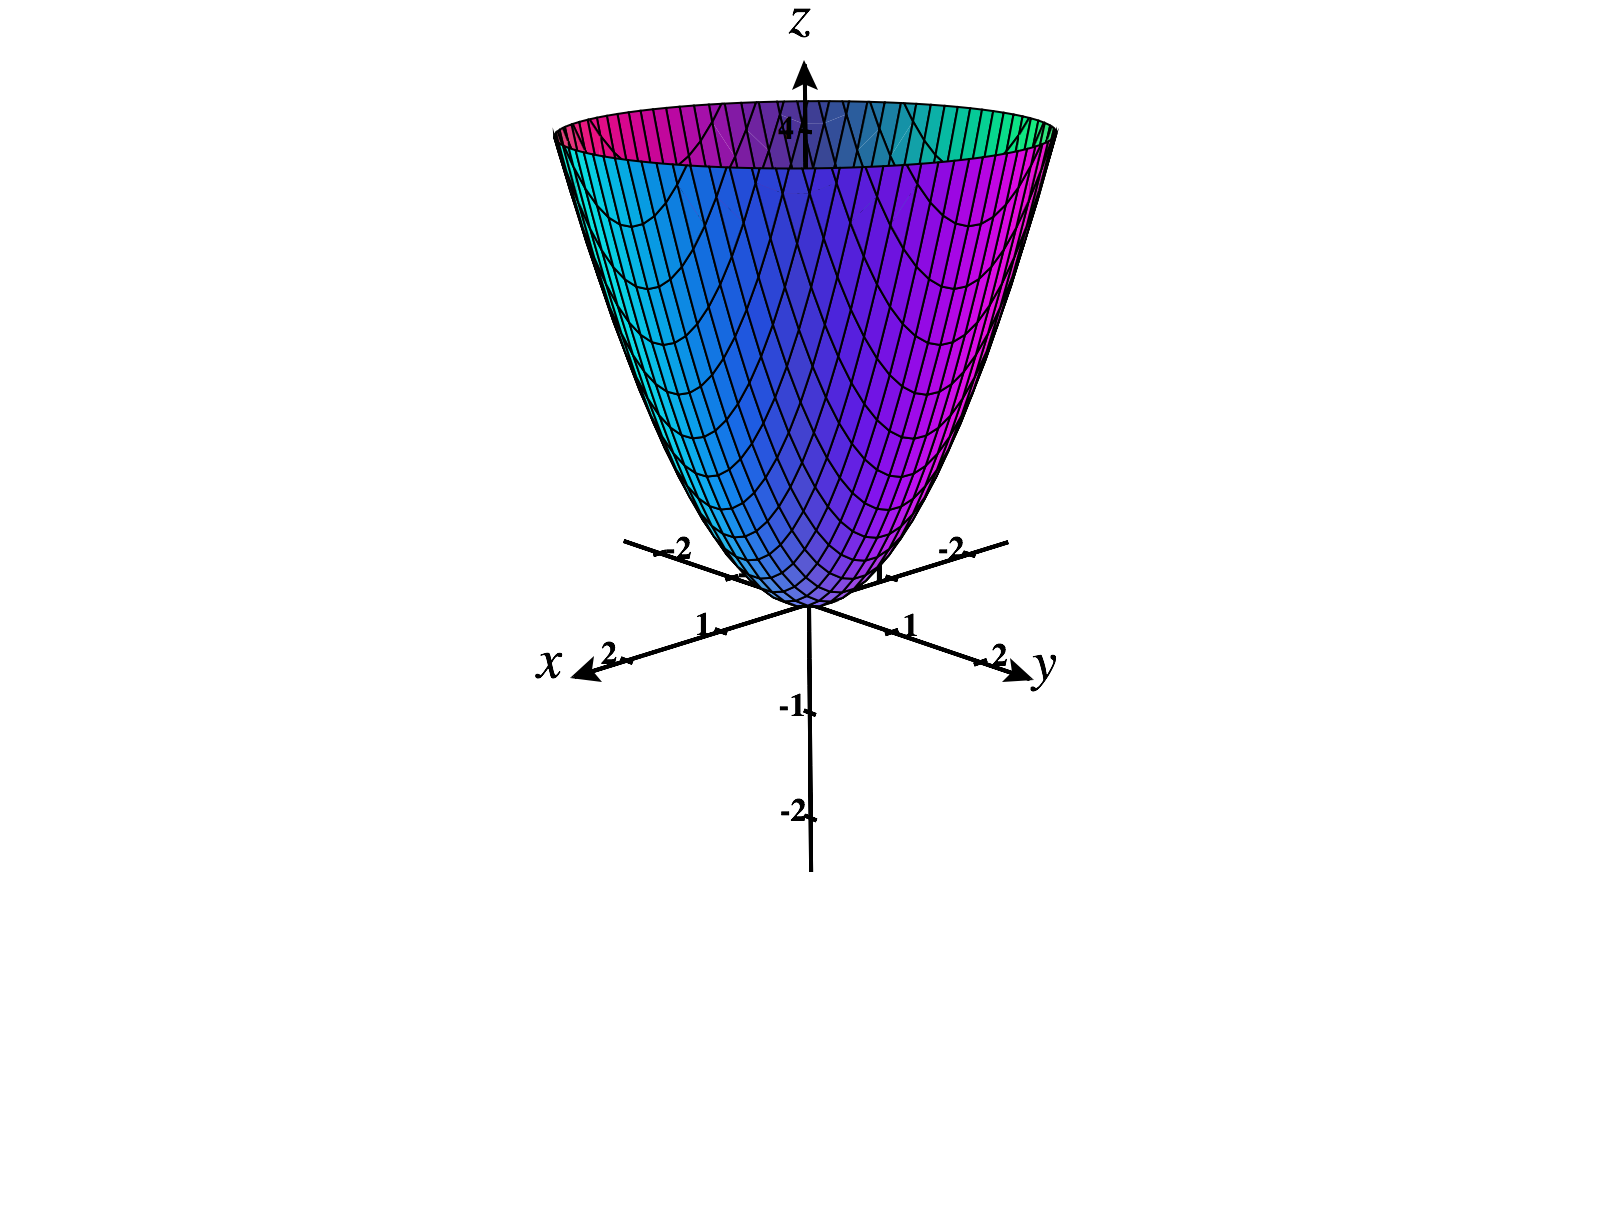
\includegraphics[width=\textwidth]{CalcPlot3D-pos_def}
\end{image}

The graphs of other positive definite quadratic forms on $\mathbb{R}^2$ look similar, though they may be stretched in various directions. Notice that for a positive definite quadratic form, there is always a strict minimum at the origin.

The quadratic form $p(x,y) = -x^2-y^2$ is negative definite. Its graph is pictured below.

\begin{image}
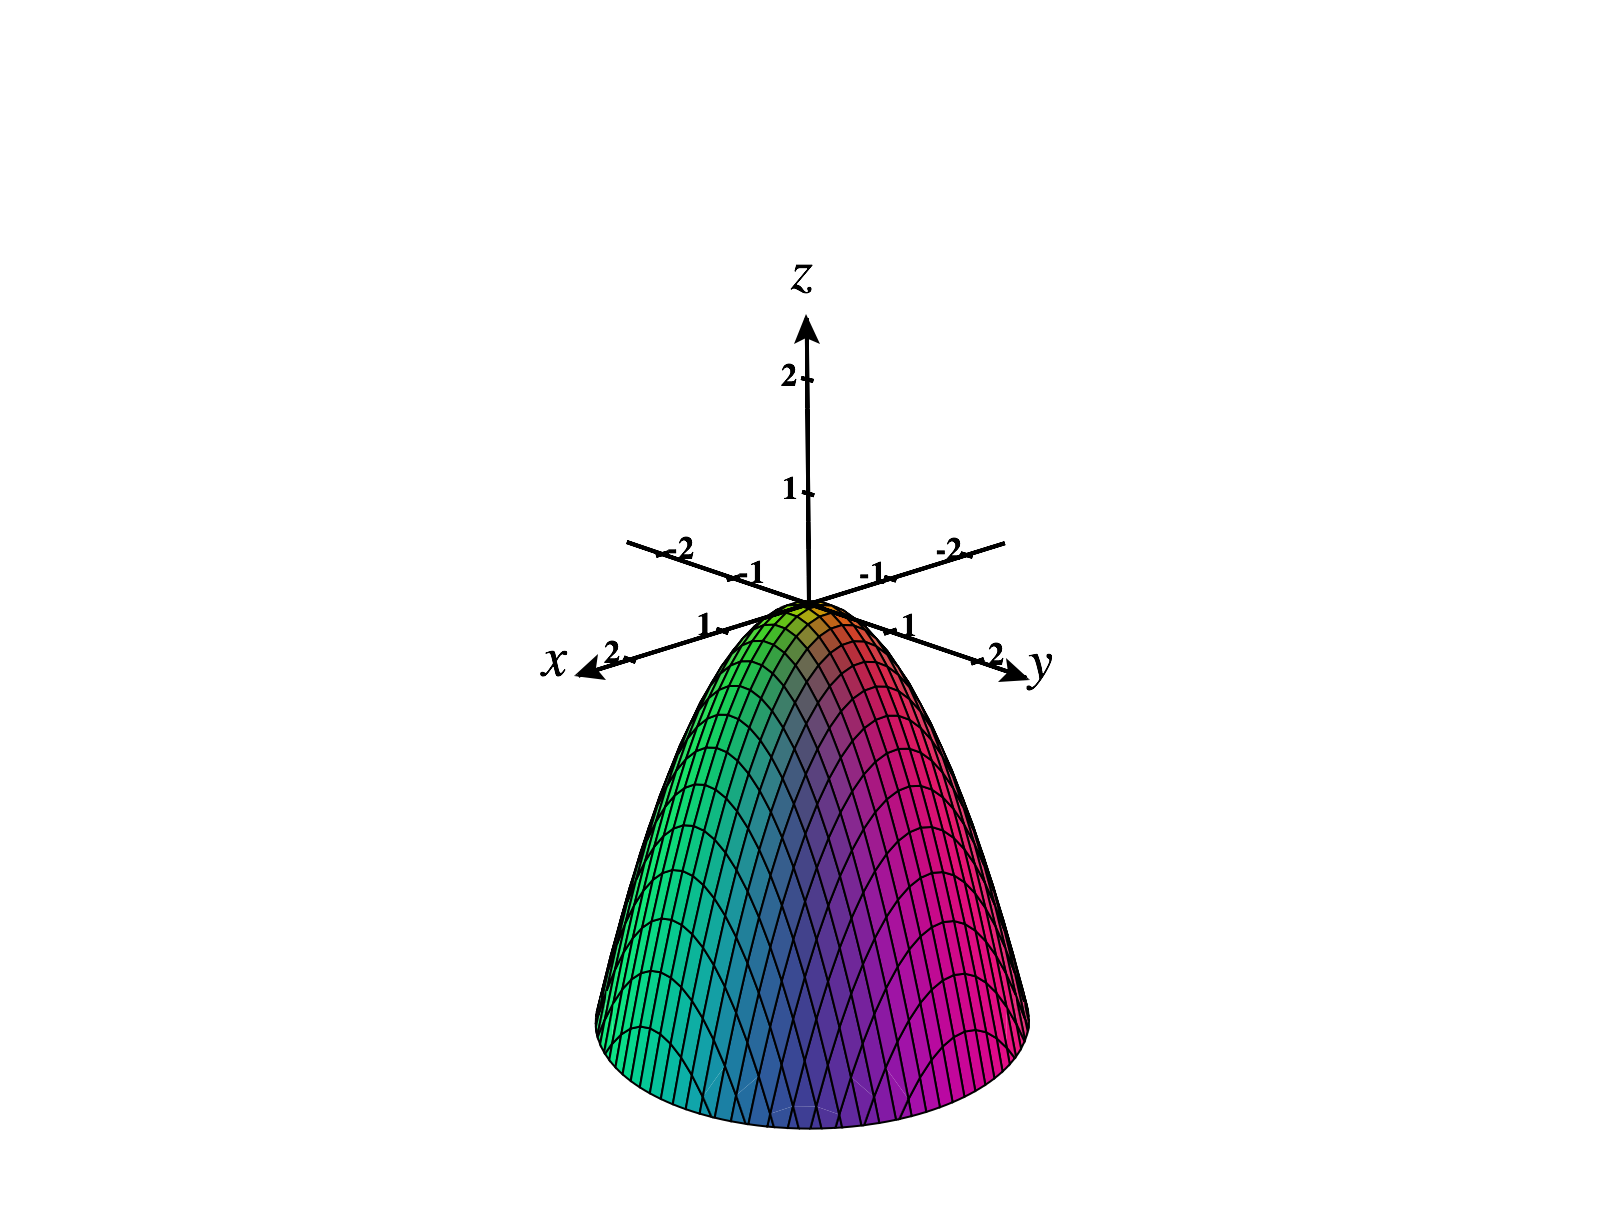
\includegraphics[width=\textwidth]{CalcPlot3D-neg_def}
\end{image}

The graphs of other negative definite quadratic forms look similar, though they may be stretched in various directions. Notice that for a negative definite quadratic form, there is always a strict maximum at the origin.

The quadratic form $p(x,y) = x^2$ is positive semi-definite. Its graph is pictured below.

\begin{image}
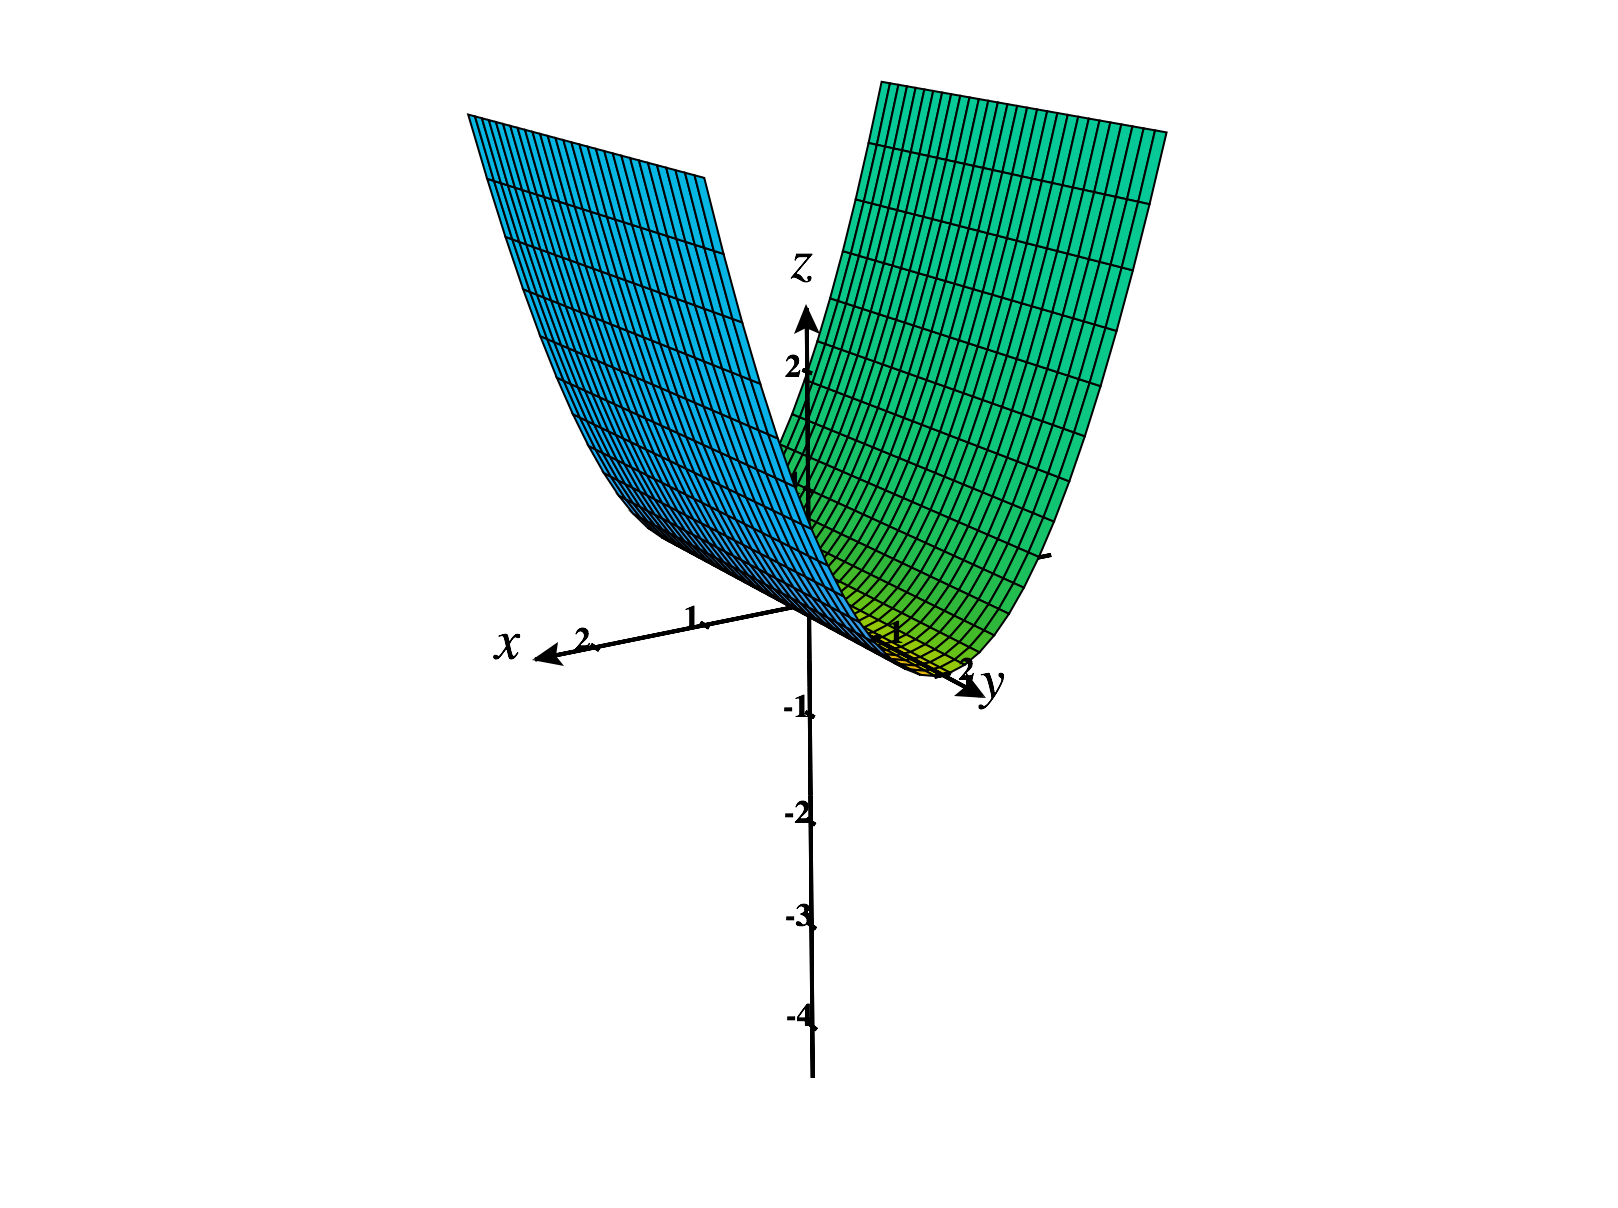
\includegraphics[width=\textwidth]{CalcPlot3D-pos_semidef}
\end{image}

The graphs of other positive semi-definite quadratic forms look similar, though they may be stretched in various directions. 

The quadratic form $p(x,y) = -x^2$ is negative semi-definite. Its graph is pictured below.

\begin{image}
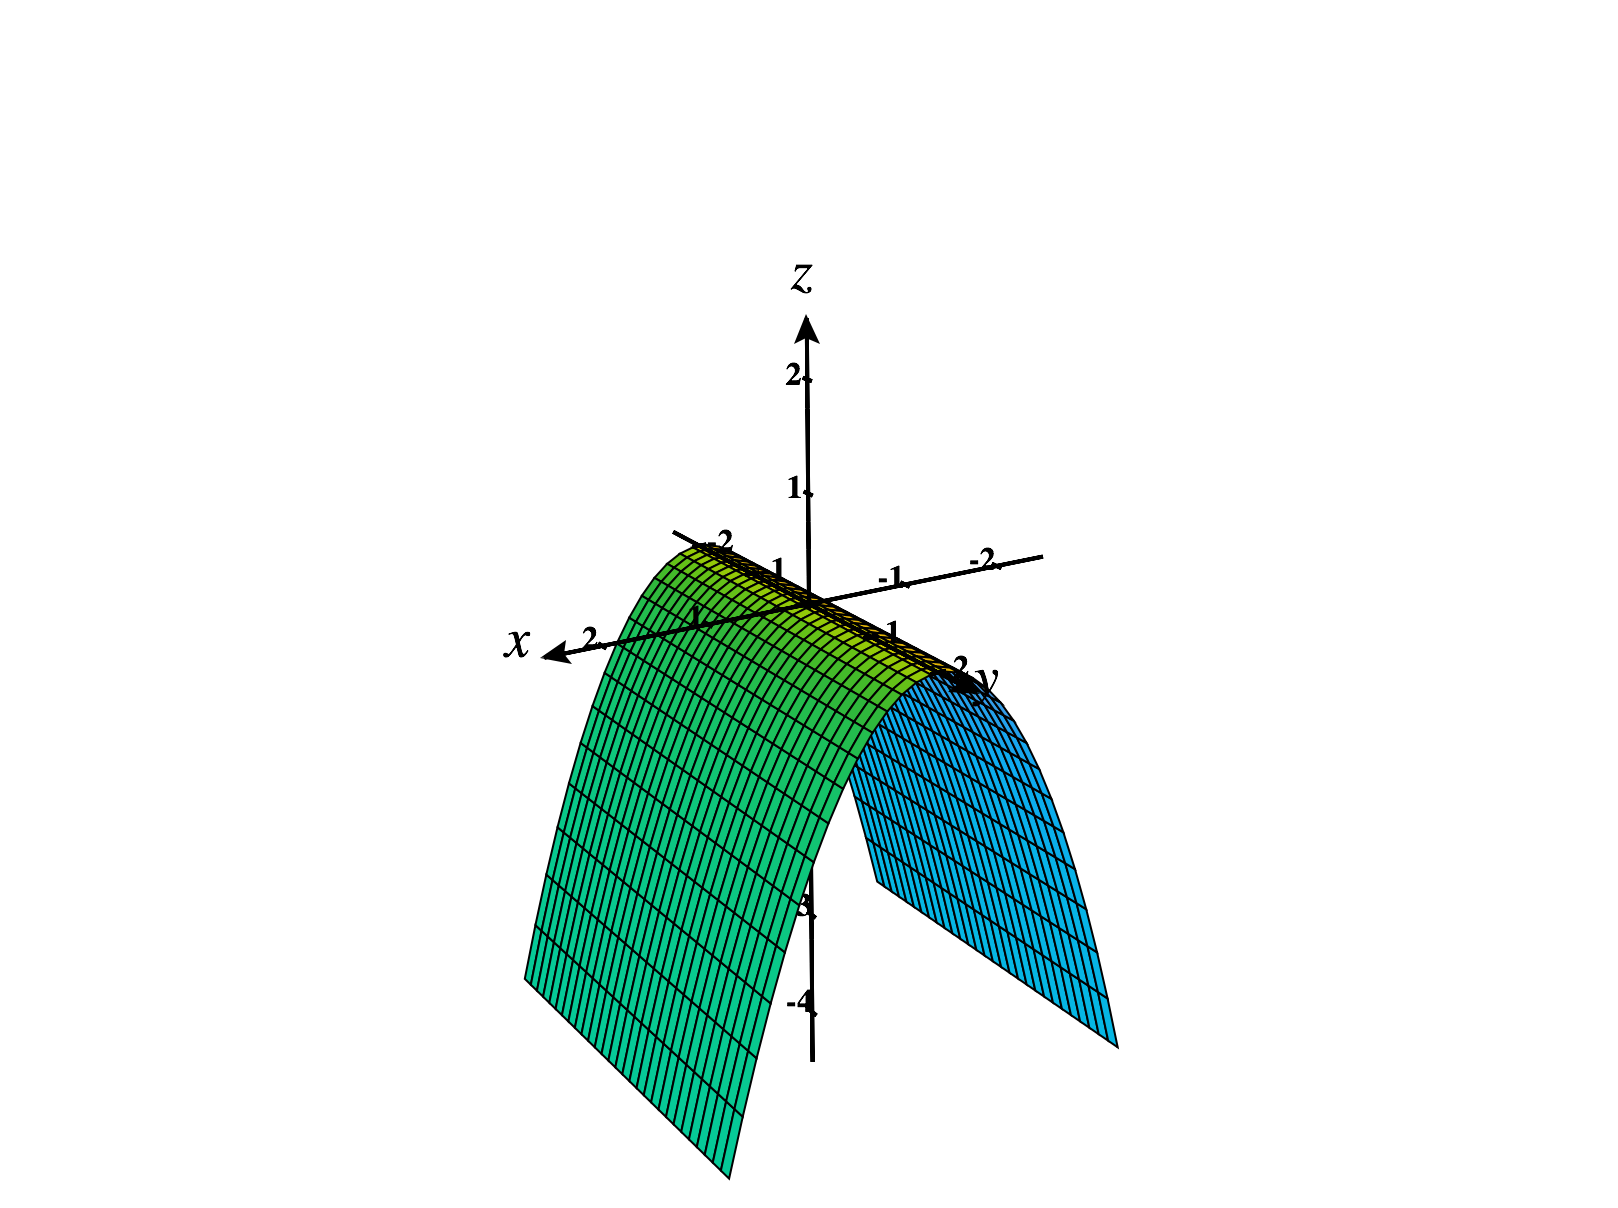
\includegraphics[width=\textwidth]{CalcPlot3D-neg_semidef}
\end{image}

The graphs of other negative semi-definite quadratic forms look similar, though they may be stretched in various directions.

The quadratic form $p(x,y) = x^2-y^2$ is indefinite. Its graph is pictured below.

\begin{image}
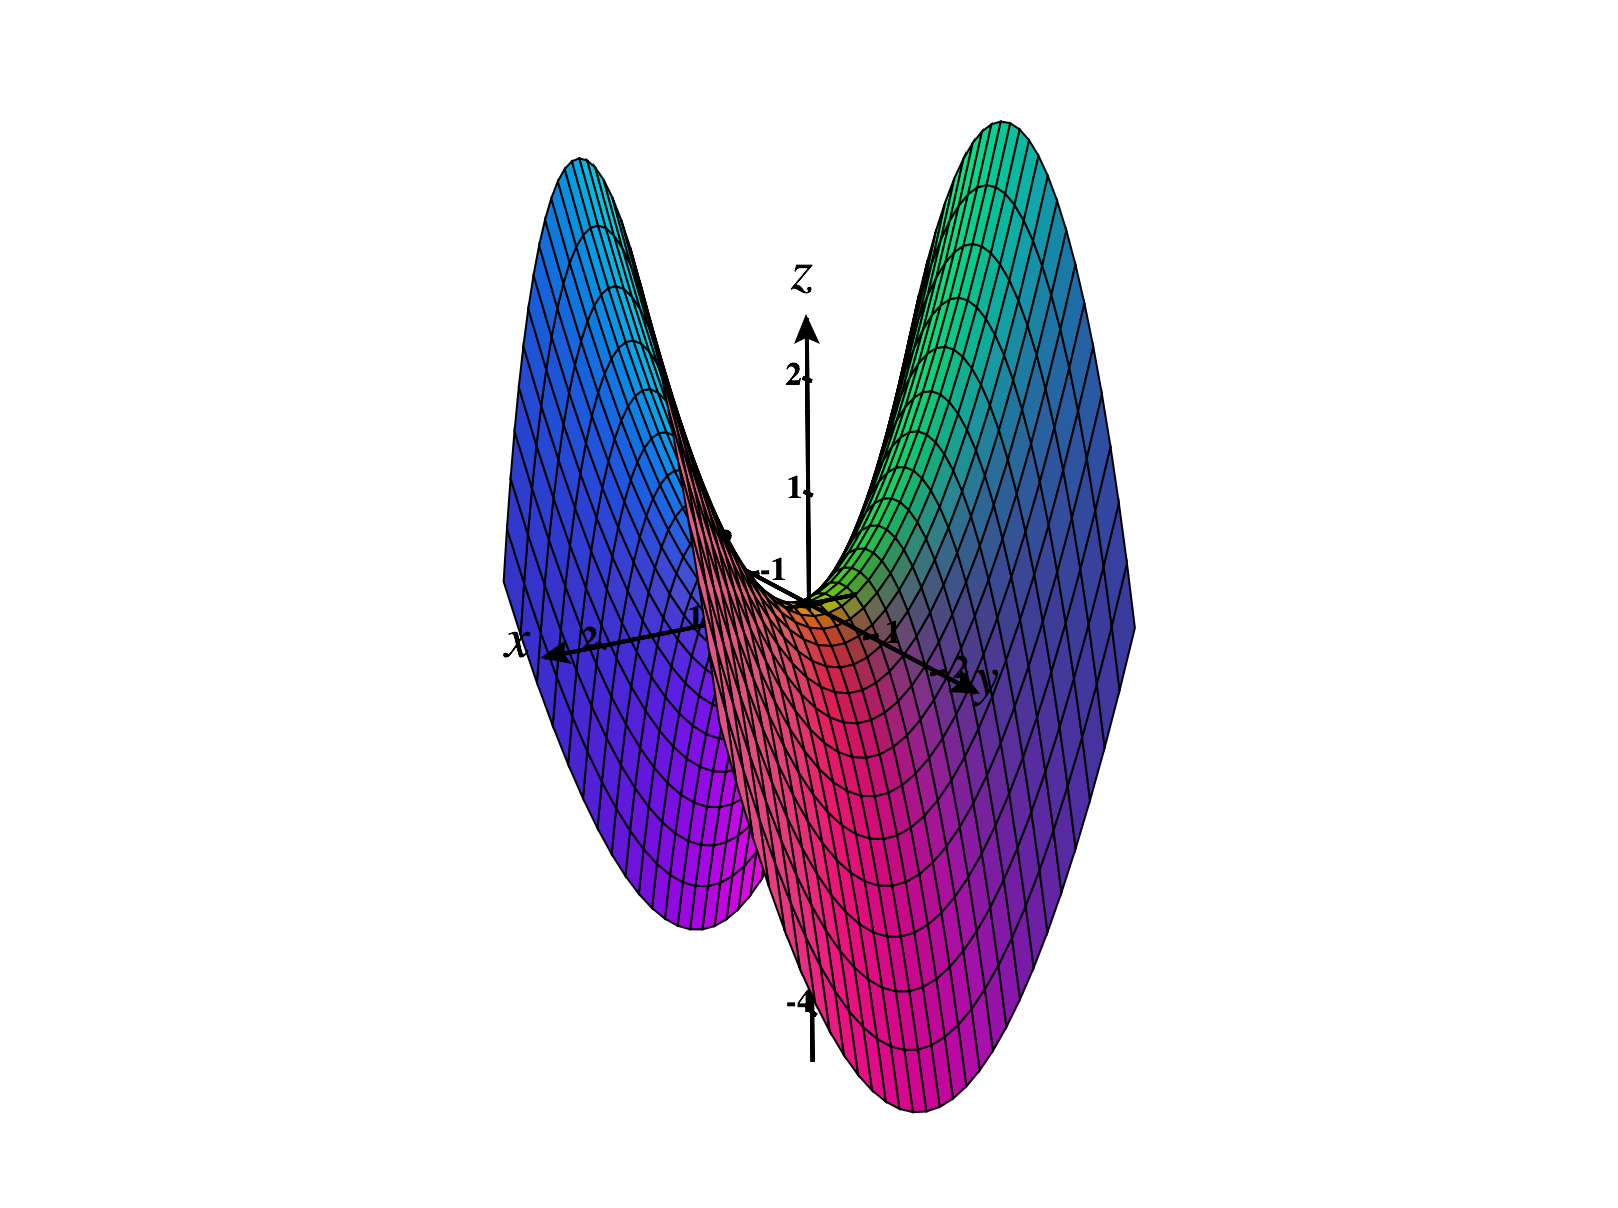
\includegraphics[width=\textwidth]{CalcPlot3D-indef}
\end{image}

The graphs of other indefinite quadratic forms look similar, though they may be stretched in various directions. Notice the behavior of the graph around the origin; because of its shape, this is called a \emph{saddle point}.

\end{example}

\section*{Sylvester's Theorem}

We can use the symmetric matrix representing a quadratic form to classify the quadratic form, by looking at a sequence of determinants.

\begin{theorem}
(Sylvester's Theorem) Let $p(\vec{x}) = \vec{x}^TA\vec{x}$, where $A$ is a symmetric matrix, 
\[
A = \begin{pmatrix}
a_{11} & a_{12} & a_{13} & \cdots & a_{1n}\\
a_{12} & a_{22} & a_{23} & \cdots & a_{2n}\\
a_{13} & a_{23} & a_{33} & \cdots & a_{1n}\\
\vdots & \vdots & \vdots & \ddots & \vdots\\
a_{1n} & a_{2n} & a_{3n} & \cdots & a_{nn}\\
\end{pmatrix}.
\]
Consider the sequence of determinants of the $n$ square upper left submatrices of $A$, 
\[
d_1 = a_{11}, d_2 = \text{det}\begin{pmatrix}a_{11} & a_{12}\\ a_{12} & a_{22}\end{pmatrix}, d_3 = \text{det}\begin{pmatrix}a_{11} & a_{12} & a_{13}\\ a_{12} & a_{22} & a_{23}\\ a_{13} & a_{23} & a_{33}\end{pmatrix},...,d_n = \text{det}\begin{pmatrix}
a_{11} & a_{12} & a_{13} & \cdots & a_{1n}\\
a_{12} & a_{22} & a_{23} & \cdots & a_{2n}\\
a_{13} & a_{23} & a_{33} & \cdots & a_{1n}\\
\vdots & \vdots & \vdots & \ddots & \vdots\\
a_{1n} & a_{2n} & a_{3n} & \cdots & a_{nn}\\
\end{pmatrix}.
\]
\begin{itemize}
\item If all of the determinants are positive, so $d_i>0$ for all $i$, then $p$ is positive definite.
\item If $d_1 < 0$, and the signed of the determinants alternate (so the odd numbered determinants are negative, and the even numbered determinants are positive), then $p$ is negative definite.
\item If all of the determinants are nonzero, but don't follow the above patterns, then $p$ is indefinite.
\end{itemize}
\end{theorem}

Notice that this theorem requires that $A$ be a symmetric matrix. Also, in the case where one or more of the determinants is zero, we can't use this theorem to classify the quadratic form.

\begin{example}
Consider the quadratic form $p(\vec{x}) = \vec{x}^T A\vec{x}$ for $A = \begin{pmatrix} -1 & 1 & -2\\ 1 & -5 & 1 \\ -2 & 1 & -10\end{pmatrix}$. Notice that $A$ is symmetric, so we'll be able to use Sylvester's Theorem. Let's find the sequence of determinants.
\begin{align*}
d_1 &= -1\\
d_2 &= \text{det}\begin{pmatrix} -1 & 1\\1 & -5\end{pmatrix}\\
&= \answer{3}\\
d_3 &= \text{det}\begin{pmatrix} -1 & 1 & -2\\ 1 & -5 & 1 \\ -2 & 1 & -10\end{pmatrix}\\
&= \answer{-23}
\end{align*}
Based on this sequence of determinants, and using Sylvester's Theorem, we have
\begin{multipleChoice}
\choice{$p$ is positive definite.}
\choice[correct]{$p$ is negative definite.}
\choice{$p$ is indefinite.}
\choice{We cannot use Sylvester's Theorem to categorize this quadratic form.}
\end{multipleChoice}
\end{example}

\begin{example}
Consider the quadratic form $p(\vec{x}) = \vec{x}^T A\vec{x}$ for $A = \begin{pmatrix} 1 & 11\\ 11 & 121\end{pmatrix}$. Notice that $A$ is symmetric, so we'll be able to use Sylvester's Theorem. Let's find the sequence of determinants.
\begin{align*}
d_1 &= \answer{1}\\
d_2 &= \text{det}\begin{pmatrix} 1 & 11\\11 & 121\end{pmatrix}\\
&= \answer{0}
\end{align*}
Based on this sequence of determinants, and using Sylvester's Theorem, we have
\begin{multipleChoice}
\choice{$p$ is positive definite.}
\choice{$p$ is negative definite.}
\choice{$p$ is indefinite.}
\choice[correct]{We cannot use Sylvester's Theorem to categorize this quadratic form.}
\end{multipleChoice}
\end{example}

\begin{example}
Consider the quadratic form $p(\vec{x}) = \vec{x}^T A\vec{x}$ for $A = \begin{pmatrix} -1 & 2 & 0\\ 0 & -4 & 0 \\ -2 & 0 & 3\end{pmatrix}$. Notice that $A$ is symmetric, so we won't immediately be able to use Sylvester's Theorem. First, we'll need to find the symmetric matrix representing $p$. Expanding $p$, we have
\begin{align*}
p(x,y,z) &= \begin{pmatrix} x & y & z\end{pmatrix}\begin{pmatrix} -1 & 2 & 0\\0 & -4 & 0\\-2 & 0 & 3\end{pmatrix}\begin{pmatrix} x \\ y\\ z\end{pmatrix}\\
&= \answer{-x^2 + 2xy - 4y^2 - 2xz + 3z^2}.
\end{align*}
From this, we can find the symmetric matrix representing $p$ to be
\[
\begin{pmatrix} -1 & 1 & -1\\ 1 & -4 & 0 \\ -1 & 0 & 3\end{pmatrix}.
\]

We now find the sequence of determinants for the symmetric matrix above.
\begin{align*}
d_1 &= -1\\
d_2 &= \text{det}\begin{pmatrix} -1 & 1\\1 & -4\end{pmatrix}\\
&= \answer{3}\\
d_3 &= \text{det}\begin{pmatrix} -1 & 1 & -1\\ 1 & -4 & 0 \\ -1 & 0 & 3\end{pmatrix}\\
&= \answer{-23}
\end{align*}
Based on this sequence of determinants, and using Sylvester's Theorem, we have
\begin{multipleChoice}
\choice{$p$ is positive definite.}
\choice{$p$ is negative definite.}
\choice[correct]{$p$ is indefinite.}
\choice{We cannot use Sylvester's Theorem to categorize this quadratic form.}
\end{multipleChoice}
\end{example}




\end{document}